\bghdr{images/fond-infobr}

\subsection{Configuration de ton navigateur \emph{Web}}
\label{browser}

\paragraph{Firefox}
\flimage{images/firefox-logo}{0.07}{l}

Lance \app{Mozilla Firefox}, et va dans le menu \menu{Outils},
\menu{Options...} (ou \menu{\'Edition}, \menu{Pr\`ef\`erences...} sous Linux). L\`a , s\'electionne la rubrique \menu{Avanc\'e}, onglet \menu{R\'eseau}, et clique sur
\menu{Param\`etres}. La case \`a  cocher est alors \menu{Adresse de configuration automatique du proxy},
et l'adresse \`a  indiquer est : \urllink{http://config/proxy.pac}.

Ensuite, il te faut accepter le certificat SSL du BR. Cela consiste \`a indiquer que tu fais confiance au BR pour authentifier les sites des binets.\\
Il suffit se se rendre sur \urllink{http://config/ca-br.crt} et de cocher toutes les cases.\\

\noindent
  \begin{figure*}[!h]
    \begin{center}  
      \subfloat[Configuration du serveur mandataire]{ 
      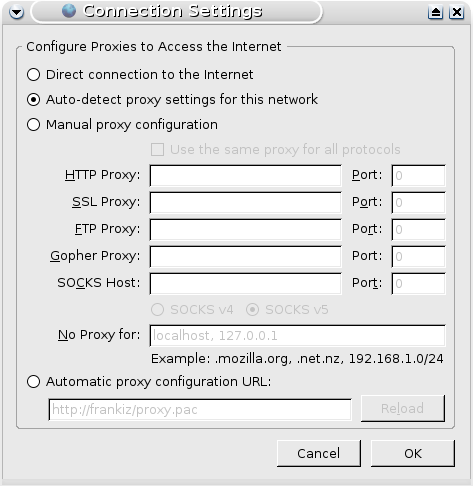
\includegraphics[width=0.48\textwidth]{images/nux_proxy_firefox}}
      \hspace{\stretch{1}}
      \subfloat[Acceptation du certificat BR]{ 
         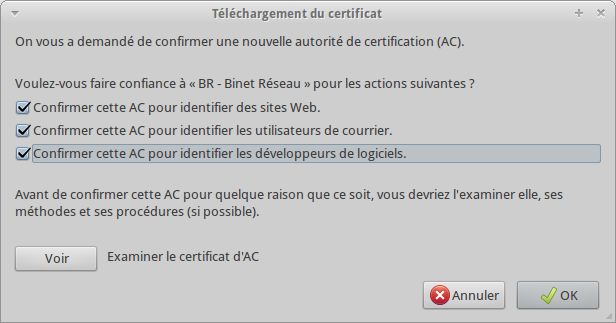
\includegraphics[width=0.48 \textwidth]{images/ca-br-ff}}
           \caption{Configuration de Firefox}
    \end{center}
  \end{figure*}
%\imagepos{images/nux_proxy_firefox}{0.65}{Configuration du serveur mandataire sous Firefox}{ht}\\
%\imagepos{images/ca-br}{1}{Acceptation du certificat BR}{ht}
%
% Pour le RTFIBRp11 pour un saut de page si n\'ec\'essaire ce qui n'\'etait pas le cas en 2008

%\noindent\rule{.4\textwidth}{.4pt}

%\vfill %\pagebreak


\paragraph{Google Chrome}
\flimage{images/google-chrome-logo}{0.07}{l}

Pour \app{Google Chrome}, la configuration du serveur mandataire se r\`egle automatique sur celle du système. Tu n'es donc pas oblig\`e de r\`egler le \emph{proxy} toi-même. Cependant, pour le faire manuellement, clique sur la
clef à molette en haut à droite, choisis \menu{Options}, va dans l'onglet \menu{Paramètres avanc\`es} (ou \menu{Under the Hood}), clique sur \menu{Modifier les paramètres du Proxy...} et règle comme ci-dessus.\\

Pour accepter le certificat BR, il te faut d'abord le t\'el\'echarger sur \urllink{http://config/ca-br.crt}.
Puis, dans Chrome, rends-toi dans \menu{Pr\'eferences}, \menu{Options avanc\`ees}, \menu{G\'erer les certificats},
\menu{Autorit\'es} et clique sur \menu{Importer}. Il suffit alors de s\'electionner l'emplacement o\`u tu avais stock\'e le certificat et de cocher toutes les cases.
\imagepos{images/ca-br-chrome}{1}{Acceptation du certificat BR sous Google Chrome}{ht}

\paragraph{Konqueror}
\flimage{images/konqueror-logo}{0.07}{l}

Sous \app{Konqueror}, cela se trouve dans le menu \menu{Configuration}, \menu{Configurer Konqueror},
dans l'onglet \menu{Serveur mandataire} ; ensuite, choisis les même r\`eglages que pour \app{Firefox} ci-dessus.
Attention : si tu ne configures pas le serveur mandataire dans Konqueror,
les logiciels KDE (\app{KGet}, \app{Adept},\dots) ne l'utiliseront pas !


%%% pas besoin de configurer au niveau navigateur sur Mac OS
%\paragraph{Safari}
%\flimage{images/mac_safari_icone}{0.07}{l}

%\app{Safari}, le navigateur web d'Apple, est maintenant compatible avec la majorit\'e des sites \emph{web}. Tu peux donc t'en servir au quotidien,
%en faisant appel \`a  \app{Firefox} pour les sites r\'ecalcitrants. 

%% CE TRUC EST PAS A SA PLACE ICI.

 % \item \app{vlc} : Un logiciel qui te permettra de recevoir la t\'el\'evision directement dans ton casert, afin d'\^etre vraiment s\^{u}r d'avoir autre chose \`a  faire que travailler les veilles de p\^ales. Configuration page \pageref{TV}.



%%%%%%%%%%%%%%%%%%%%%%%%%%%%%%%%%%%%%%%%%%%%%%%%%%%%%%%%%%%%%%%%%%%%
%                            MAIL                                  %
%%%%%%%%%%%%%%%%%%%%%%%%%%%%%%%%%%%%%%%%%%%%%%%%%%%%%%%%%%%%%%%%%%%%

\subsection{Configuration de ton client \emph{mail}}

La DSI met \`a  ta disposition une bo\^{i}te aux lettres \'electronique sur
le serveur \server{poly} ; cette section t'explique comment
configurer \app{Windows Mail}, \app{Kmail} et \app{Mac OS Mail} pour y avoir acc\`es. Tu peux bien
s\^{u}r utiliser \app{Thunderbird} si tu pr\'ef\`eres, les donn\'ees \`a  rentrer
pour la configuration sont les m\^emes ; quelques d\'etails sont donn\'es
dans le WikiX sur \fkz. De plus, tu trouveras des explications plus
d\'etaill\'ees dans le manuel r\'edig\'e par la DSI.

\paragraph{Outlook et Windows Mail}
\flimage{images/outlook-logo}{0.07}{l}

La proc\'edure suivante fonctionne aussi avec \app{Windows Mail}.
Lance \app{Outlook Express} et va dans le menu \menu{Outils},
\menu{Comptes\ldots}. Clique sur le bouton \menu{Ajouter\ldots} en
haut \`a  droite, puis sur \menu{Courrier\ldots}.

Pour \app{Windows Mail} c'est sur compte de messagerie qu'il faut cliquer, avant de cliquer sur suivant.

Remplis les \'ecrans de configuration avec les donn\'ees suivantes.
\begin{description}
  \item[Nom complet : ] ton nom (\guillemotleft~Martin Durand~\guillemotright , par exemple)
  \item[Adresse de messagerie : ] de la forme \mail{prenom.nom@polytechnique.edu}
  \item[Type de serveur de messagerie pour le courrier entrant : ] \menu{POP3}
  \item[Serveur de messagerie pour le courrier entrant : ] \server{poly.polytechnique.fr}
  \item[Serveur de messagerie pour le courrier sortant : ] \server{poly.polytechnique.fr} ou \newline \server{ssl.polytechnique.org}
  \item[Nom du compte : ] ton identifiant \server{poly} (en g\`en\`eral c'est \texttt{prenom.nom}, si ça ne marche pas, va voir le bureau \emph{login} de la DSI.)
  \item[Mot de passe : ] ton mot de passe \server{poly}
       v\'erifie bien que la case \menu{M\'emoriser le mot de passe} est coch\'ee.
\end{description}

Voil\`a , clique sur \menu{Continuer}, \menu{Terminer}.

Tu te retrouves alors sur la fen\^etre \menu{Comptes Internet}. Va sur
l'onglet \menu{Courrier}, clique sur le compte que tu viens de cr\'eer
puis sur \menu{Propri\'et\'es}. Clique sur l'onglet \menu{Avanc\'e} et
configure comme sur la capture~\ref{config:win:mail} ; en
particulier, coche la seconde case \menu{Ce serveur n\'ecessite une
connexion s\'ecuris\'ee (SSL)}.

Comme \c{c}a, tu peux d\'esormais recevoir des \emph{mails} avec une liaison
s\'ecuris\'ee vers \server{poly} pour que personne ne puisse les
intercepter. Il est possible que tu aies à accepter manuellement le certificat utilis\`e par l'\'Ecole pour que cela fonctionne correctement. Tu le trouveras sur \urllink{http://poly}. Une fois t\'el\'echarg\'e, il suffit de l'importer.

\imageref{images/win_config_mail_avance}{0.5}{Configuration avanc\'ee
des serveurs \emph{mail}}{!h}{config:win:mail}



\paragraph{Kmail}
\flimage{images/kmail-logo}{0.07}{l}

Pour \app{Kmail}, va dans \menu{Configuration}, \menu{Configurer Kmail}. Choisis la
rubrique \menu{Comptes}. Commence par cr\'eer un nouveau compte dans
l'onglet \menu{R\'eception des messages} en cliquant sur le bouton
\menu{Ajouter\ldots} et choisis le type POP3.


\noindent
  \begin{figure*}[!h]
    \begin{center}  
      \subfloat[R\'eception des messages]{ 
      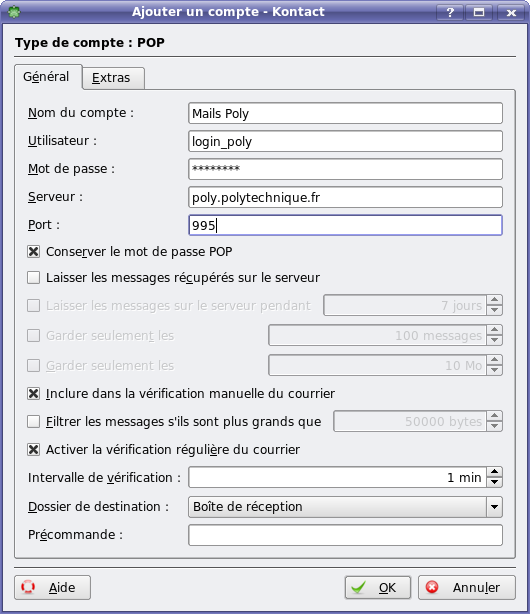
\includegraphics[width=0.48\textwidth]{images/nux_config_kmail_pop} }
      \hspace{\stretch{1}}
      \subfloat[Envoi des messages]{ 
 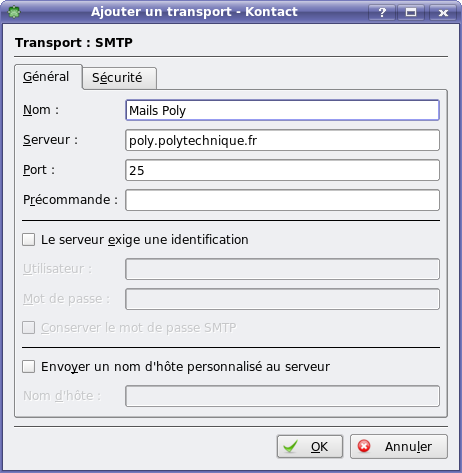
\includegraphics[width=0.48 \textwidth]{images/nux_config_kmail_smtp} }
 \caption{Configuration sous \app{Kmail}}
    \end{center}
  \end{figure*}


Utilise les param\`etres suivants pour configurer l'onglet \menu{G\'en\'eral}.
\begin{description}
  \item[Nom : ] le nom du compte, par exemple : Mails Poly
  \item[Utilisateur : ] l'identifiant \server{poly} que t'a fourni la DSI \`a  ton arriv\'ee sur le plateau
  \item[Mot de passe : ] le mot de passe \server{poly}
  \item[Serveur : ] \server{poly.polytechnique.fr}
  \item[Port : ] 995
\end{description}
Ensuite, va dans l'onglet \menu{Extras} et coche la case
\menu{Utiliser SSL pour s\'ecuriser les t\'el\'echargements}.

Maintenant, dans l'onglet \menu{Envoi des messages} clique sur le
bouton \menu{Ajouter\ldots}. Utilise les param\`etres suivants pour le
configurer :
\begin{description}
  \item[Nom] le m\^eme nom de compte que pr\'ec\'edemment
  \item[Serveur] \server{poly.polytechnique.fr} ou \server{ssl.polytechnique.org}
  \item[Port] 25
\end{description}
Sinon, laisse toutes les cases d\'ecoch\'ees.

%Tu peux aussi configurer l'acc\`es \`a  \app{l'annuaire LDAP} de l'\'Ecole, sorte de carnet d'adresses en ligne qui contient les adresses \emph{mail} de tout le monde sur le campus. Pour ce faire, commence par ouvrir \menu{Outils}, \menu{Carnet d'adresses}, puis va dans \menu{Configuration}, \menu{Configurer kAdressBook}, \menu{Consultation LDAP}. Clique ensuite sur \menu{Ajouter un h\^ote}, et configure comme suit: \\
%\smallskip
%\begin{minipage}[t]{0.48\textwidth}
%\begin{description}
%  \item[H\^ote] \server{ldap.eleves.polytechnique.fr}
%  \item[Port] 389
%  \item[Version de LDAP] 3
%\end{description}  
%\end{minipage} 
%\begin{minipage}[t]{0.48\textwidth}
%\begin{description}  
%  \item[DN] \server{dc=polytechnique, dc=ldap, dc=eleves, dc=fr}
%  \item[S\'ecurit\'e] Non
%  \item[Identification] Anonyme
%\end{description}
%\end{minipage} \\
%Une fois revenu dans \menu{Configuration LDAP}, coche la case \server{ldap.eleves.polytechnique.fr}. Tu as maintenant acc\`es \`a  l'annuaire LDAP lors de la
%r\'edaction de messages, avec tout au plus un red\'emarrage de \app{Kmail}. 
%
%\imagepos{images/nux_config_ldap}{0.55}{Configuration de l'annuaire LDAP sous Kmail}{pht}
%\imagepos{images/nux_config_knode}{0.45}{Configuration de Knode}{ht}
%
%\noindent
%  \begin{figure*}[!h]
%    \begin{center}  
%      \subfloat[Configuration de l'annuaire LDAP sous Kmail]{ 
%      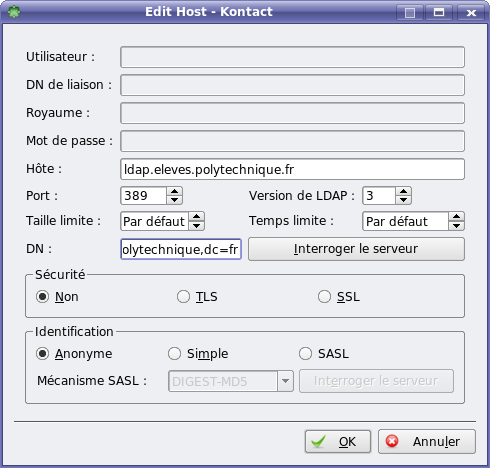
\includegraphics[width=0.48\textwidth]{images/nux_config_ldap}}
%      \hspace{\stretch{1}}
%      \subfloat[Configuration de Knode]{ 
% 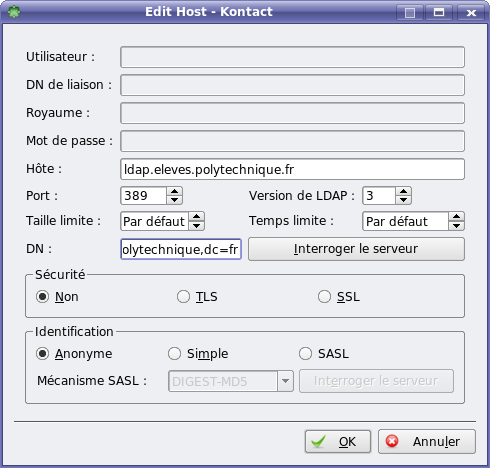
\includegraphics[width=0.48 \textwidth]{images/nux_config_ldap} }
% \caption{Configurations LDAP et \emph{news}}
%    \end{center}
% \end{figure*}


\paragraph{Mac OS Mail}

\flimage{images/mac_mail_icone}{0.07}{l} \app{Mail} : un client \emph{mail} offrant les fonctionnalit\'es classiques d'un bon client : recherche instantan\'ee, filtre antispam, r\`egles de tri automatique des \emph{mails}, regroupement des \emph{mails} correspondant \`a  une m\^eme discussion.

Au premier lancement, \app{Mail} te demandera de remplir les informations concernant ton compte \emph{mail} sur \server{poly}, il suffit de le remplir avec les donn\'ees suivantes :
\begin{description}
  \item[Nom complet] ton nom !
  \item[Adresse \'electronique] de la forme \mail{prenom.nom@polytechnique.edu}
  \item[Serveur de r\'eception] \server{poly.polytechnique.fr}
  \item[Type de compte] \menu{POP}
  \item[Nom d'utilisateur] ton \emph{login} \server{poly} (les huit premi\`eres lettres de ton nom en g\'en\'eral)
  \item[Mot de passe] ton mot de passe \server{poly}
  \item[Serveur d'envoi (SMTP)] \server{poly.polytechnique.fr} ou \server{ssl.polytechnique.org}
\end{description}

Si tu as d\'ej\`a  cr\'e\'e un compte pr\'ec\'edemment, il faut aller dans les \menu{Pr\'ef\'erences} (accessibles depuis le menu \menu{Mail}), onglet \menu{Comptes}, pour cr\'eer un autre compte en cliquant sur la case \menu{+}.

N'oublie pas de cocher \menu{Activer le cryptage SSL} dans l'onglet \menu{Avanc\'e}, port 995. Tu souhaiteras alors certainement installer le certificat de s\'ecurit\'e de \server{poly} (tu le trouveras sur \urllink{http://poly/}). Une fois que tu as t\'el\'echarg\'e le certificat, ouvre le fichier \menu{.CRT} obtenu, et dans \app{Trousseau d'acc\`es}, installe-le dans %\menu{X509Anchors} (Tiger) ou 
\menu{session} (Leopard).

Cette configuration marche pour acc\'eder \`a  ses mails depuis l'int\'erieur de l'X mais aussi de l'ext\'erieur, sans rien changer.
En revanche tu ne peux pas envoyer de \emph{mails} depuis l'ext\'erieur, car le serveur \server{poly} ne le permet pas.
Nous te conseillons vivement d'utiliser le serveur SMTP \server{polytechnique.org} et de regarder la configuration propos\'ee par \urllink{Polytechnique.org}.
Celle-ci permet d'envoyer des \emph{mails} \`a  l'ext\'erieur de l'\'Ecole de façon s\`ecuris\`ee, sans modifier ta configuration par la suite.
Tu peux ajouter ce SMTP dans l'onglet \menu{Comptes} des \menu{Pr\'ef\'erences} de \emph{mail} et r\'egler dans l'onglet \menu{Avanc\'es} comme dans la capture.

\begin{figure*}[!hl]
    \begin{center}
            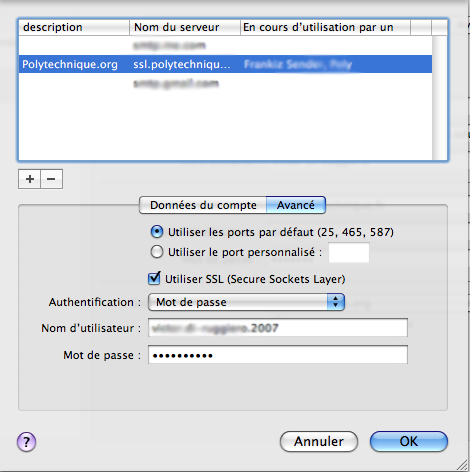
\includegraphics[width=0.4\textwidth]{images/mac_config_smtp_poltechnique.png} 
      \caption{Configurer le serveur SMTP \server{Polytechnique.org}}
    \end{center}
  \end{figure*}

%Le LDAP ne fonctionne pas \`a  l'heure actuelle avec \app{Mail} (mars 2009) sous \app{Leopard}, contrairement aux  autres syst\`emes d'exploitation (fonctionne cependant avec \app{Thunderbird}).
%\subsuEnfin, tu peux disposer dans \app{Mail} de l'annuaire de l'\`acole, mis \`a  disposition par la DSI. Pour cela, va dans les \menu{Pr\'ef\'erences} de Mail,
%puis dans la rubrique \menu{R\'edaction} et clique sur \menu{Configurer LDAP\ldots}. Tu peux ensuite utiliser le bouton \menu{+} pour ajouter un
%serveur, et remplir la fen\^etre comme sur la capture.

%\imagepos{images/mac_config_ldap}{0.6}{Configurer l'annuaire}{!ht}
%bsection{Logiciels additionnels}

%Les logiciels suivants sont utiles pour utiliser avec Mac OS X les services propos\'es sur le r\'eseau ; ils sont t\'el\'echargeables sur \server{frankiz}, dans la rubrique \menu{T\'el\'echarger}, \menu{Mac}.



%%%%%%%%%%%%%%%%%%%%%%%%%%%%%%%%%%%%%%%%%%%%%%%%
% ANCIENNE CONFIGURATION DES BR POUR CHAQUE OS %
%%%%%%%%%%%%%%%%%%%%%%%%%%%%%%%%%%%%%%%%%%%%%%%%

%% VIEILLE PAGE DE CONF NEWSGROUP POUR WINDOWS

%\subsubsection{Configuration \emph{newsgroups}}
%
%Reporte-toi a la page~\pageref{newsgroups} pour la description et des d\'etails de fonctionnement des \emph{newsgroups} \`a  l'X.
%
%Comme pour les \emph{mails}, nous d\'ecrivons la configuration de \app{Outlook Express} mais elle est sensiblement \'equivalente pour \app{Thunderbird}. Lance
%\app{Outlook Express} et va dans le menu \menu{Outils}, \menu{Comptes\ldots}. Clique sur le bouton \menu{Ajouter\ldots} en haut \`a  droite,
%\menu{News\ldots}. Remplis les \'ecrans de configuration suivants avec ces donn\'ees :
%\begin{description}
%  \item[Nom complet] ton nom !
%  \item[Adresse de messagerie] de la forme \mail{prenom.nom@polytechnique.edu}
%  \item[Serveur de news (NNTP)] \server{news} ; v\'erifie \`a  ce moment que la case
%       \menu{Connexion \`a  mon serveur de news requise} n'est pas coch\'ee.
%\end{description}
%Voil\`a , clique sur \menu{Continuer}, \menu{Terminer}; tu es abonn\'e
%au serveur \emph{news} des \'el\`eves.
%
%Quand tu fermeras la fen\^etre `Comptes Internet', il va te demander \`a 
%quels \emph{newsgroups} tu veux t'abonner, tu n'auras qu'\`a  s\'electionner
%ceux qui t'int\'eressent. Reporte-toi \`a  la page \pageref{newsgroups}
%pour plus d'infos sur les newsgroups auxquels t'abonner !
%
%Si tu veux t'inscrire \`a  d'autres serveurs \emph{news}, refais cette
%proc\'edure en rentrant le nom du serveur qui t'int\'eresse \`a  la place
%de \fkz.
%\setcounter{page}{12}

%% VIEILLE PAGE DE CONF NEWSGROUPS POUR LINUX


%\subsubsection{Configuration \emph{news}}
%
%\flimage{images/nux_knode_icon}{0.12}{l} Le client \emph{news} le plus utilis\'e est \app{Knode}. Parmi les autres clients \emph{news}, citons 
%\app{Thunderbird}, \app{Pan} ou \app{slrn}. Ici aussi, la configuration est presque ind\'ependante du logiciel choisi.
%
%
%Sous \app{Knode}, c'est dans le menu \menu{Configuration}, puis \menu{Configurer Knode}. Va dans la rubrique \menu{Comptes, Forums de discussion} et
%cr\'ee un compte en cliquant sur \menu{Ajouter\ldots}.
%
%\imagepos{images/nux_config_knode}{0.45}{Configuration de Knode}{ht}
%
%\pagebreak
%
%Remplis l'onglet \menu{Serveur} avec les informations suivantes :
%\begin{description}
%  \item[Nom] ce que tu veux pour d\'ecrire ce compte, par exemple 'News Frankiz'
%  \item[Serveur] \server{news}
%\nopagebreak  \item[Port] 119
%\end{description}
%
%\pagebreak
% 
%Ensuite occupe-toi de l'onglet \menu{Identit\'e} :
%\begin{description}
%  \item[Nom] mets ton pseudo dans ce champ
%  \item[Organisation] X, \'Ecole polytechnique, comme tu le sens
%  \item[Adresse \'electronique] ton adresse \emph{mail}, pour que les gens puissent te r\'epondre par \emph{mail}.
%\end{description}
%
%Enfin, pour que \app{Knode} puisse envoyer des \emph{mails}, il faut aller
%dans la rubrique \menu{Comptes}, sous-rubrique \menu{Serveur de
%courrier (SMTP)}, et choisir comme serveur d'envoi de \emph{mails}
%\server{poly.polytechnique.fr}, port 25 --- c'est exactement la m\^eme
%configuration SMTP que \app{Kmail}.
%
%Si tu veux mettre une signature \`a  la fin des messages que tu
%posteras, il te suffit de la mettre dans l'onglet \menu{Identit\'e}.
%Sur la plupart des clients la signature est interpr\'et\'ee comme
%ext\'erieure au message et n'est en particulier pas incluse dans le
%texte cit\'e lorsque tu r\'eponds \`a  un message. Pour d\'efinir une
%signature \`a  la main, il suffit de mettre \verb*+-- +\ (c'est \`a  dire
%-{}-<espace>) sur une ligne, et tout ce qui suivra cette ligne
%composera ta signature.
%
%Il ne te reste plus qu'\`a  t'inscrire \`a  des \emph{newsgroups} (reporte-toi \`a  la page \pageref{newsgroups} pour plus d'infos) et \`a  poster ! \\
%
%Pour te connecter aux serveurs de \emph{news} de Polytechnique.org, qui ont un acc\`es s\'ecuris\'e, avec \app{Knode}, il y a une petite subtilit\'e car il
%ne g\`ere pas le SSL. Il faut installer \app{stunnel} qui permet de d\'efinir une redirection SSL de port. Dans \file{/etc/stunnel.conf} (ou parfois \file{/etc/stunnel/stunnel.conf}), mets les lignes suivantes (les trois premi\`eres y sont en principe d\'ej\`a ) :
%\cmdline{\# location of pid file\\
%pid = /etc/stunnel/stunnel.pid\\
%\\
%\# user to run as\\
%setuid = stunnel\\
%setgid = stunnel\\
%\\
%\# Use it for client mode\\
%client = yes\\
%\\
%\# sample service-level configuration\\
%{[}nntps{]}\\
%accept  = 1119\\
%connect = ssl.polytechnique.org:563\\
%TIMEOUTclose = 0
%}
%
%Il ne te reste plus qu'\`a  lancer \app{stunnel} par :
%\cmdline{/etc/init.d/stunnel start}
%
%Et tu peux ainsi lire les \emph{news} de Polytechnique.org en mettant \server{localhost} comme serveur et
%\server{1119} comme port. Il faut aussi que tu coches \menu{Le serveur exige une identification} et
%que tu rentres ton nom d'utilisateur \`a  Polytechnique.org et ton mot de passe, que tu peux d\'efinir
%sur \urllink{https://www.polytechnique.org/Xorg/SMTPSecurise}.

%% VIEILLE PAGE DE CONF NEWSGROUP POUR MAC


%\subsubsection{Configuration \emph{news}}
%
%\flimage{images/mac_thunderbird_icone}{0.07}{l} 
%\app{Thunderbird} : un client \emph{news} permettant d'acc\'eder aux forums de discussion des \'el\`eves (voir page~\pageref{newsgroups} pour les d\'etails sur \server{frankiz}), mais aussi \`a  ceux de \server{usenet} gr\^ace au serveur \server{polynews.polytechnique.fr}. Il est tr\`es proche d'\app{Outlook Express} dans son esprit. Dans la m\^eme cat\'egorie, il existe \app{MacSOUP}, \app{Unison} ou encore \app{MT-NewsWatcher}. La configuration se fait de la m\^eme mani\`ere.
%
%Au premier lancement, l'application te propose d'importer les param\`etres depuis une autre application. Clique sur \menu{Suivant}. Tu peux alors choisir quel type de compte tu veux configurer (tu remarqueras que tu peux aussi cr\'eer un compte courrier \'electronique, et un compte RSS). S\'electionne \menu{Compte forums de discussion} et clique sur \menu{Suivant}. Entre alors les informations suivantes :
%
%\begin{description}
%  \item[Votre nom] ton nom ou ton pseudo
%  \item[Adresse de courrier] \mail{prenom.nom@polytechnique.edu}
%  \item[Serveur de forums] \server{news}
%  \item[Nom du compte] News Frankiz
%  \item[Nom d'utilisateur] ton \emph{login }poly (les huit premi\`eres lettres de ton nom en g\'en\'eral)
%  \item[Serveur d'envoi (SMTP)] \server{poly.polytechnique.fr} ou \server{ssl.polytechnique.org}
%\end{description}
%
%
%Pour t'abonner \`a  des groupes de discussion, il te suffit de s\'electionner le compte \menu{News Frankiz} dans la fen\^etre \menu{Dossiers} de \app{Thunderbird}, puis de cliquer sur \menu{G\'erer les abonnements aux groupes de discussion}. Tu pourras ensuite s\'electionner les forums qui t'int\'eressent parmi la liste propos\'ee. Reporte-toi \`a  la page \pageref{newsgroups} pour plus d'infos sur les \emph{newsgroups} auxquels t'abonner !
%
